% %~% %~% %~% %~% %~% %~% %~% %~% %~% %~% %~% %~% %~% %~%
%
% Here we answer the question: What did we find? It
% is here that we document the findings and the evidence
% for them. Given the importance of longitudinal analysis
% for us, it is here that we document changes with time.
%
% %~% %~% %~% %~% %~% %~% %~% %~% %~% %~% %~% %~% %~% %~%
\section{Revisiting assumptions}
\label{section:rate:analysis}

%\renewcommand{\thesubsectiondis}{Assumption \Alph{subsection}.}
Having processed each daily trace individually, flow characteristics are aggregated longitudinally in order to trace the evolution of constraints affecting \ac{TCP} across time and both spatial and topological dimensions, following the process described in section \ref{section:malawi:dataset}.
The ensuing analysis revisits four commonly held assumptions regarding Internet throughput. 
The aim in doing so is to provide a much needed factual verification of these assumptions, which itself can lead to a re-appraisal of Internet throughput modelling efforts, particularly those enunciated in Zhang et al.\ \cite{Zhang:2002p85}.
Although all models require simplifying assumptions in the name of analytic tractability, the primary goal of this section is to inform on which are the best assumptions to make if one is setting out to use or develop an Internet traffic throughput model. 

\subsection{Throughput is primarily shaped by \acs{TCP}}

% define the assumption
Internet flow rates are commonly viewed as the output of congestion control embedded at the transport layer. While it is often convenient to model flow throughput according to the steady state behaviour of such algorithms, there are many potential caveats.
For one, there is an implicit assumption that the network is the bottleneck. Under such conditions, \ac{TCP} acts as a distributed optimisation algorithm in allocating capacity to flows. Section \ref{section:rate:flow} however presented several cases where such an assumption does not hold. The prevalence of application pacing, host limitations or receiver shaping can all condition the accuracy of models which assume only elastic traffic adjusting to network conditions alone.

% explore the results
\begin{table}\footnotesize
\centering
     \begin{tabular}{  p{1.0cm} 
>{\centering\arraybackslash}p{1.0cm} 
>{\centering\arraybackslash}p{1.0cm} 
>{\centering\arraybackslash}p{1.0cm} 
>{\bfseries\centering\arraybackslash}p{1.0cm} 
>{\centering\arraybackslash}p{1.0cm} }

& \multicolumn{4}{c}{Limitation (\%)} \\
\cline{2-5}
Year & Application & Host & Receiver & Total & Loss (\%)\\

\hline

     2007 & 49.47 & 18.58 & 0.55 & 68.60 & 1.29 \\2008 & 49.55 & 17.80 & 0.69 & 68.04 & 1.37 \\2009 & 47.10 & 14.50 & 2.57 & 64.17 & 1.44 \\2010 & 36.78 & 20.44 & 3.21 & 60.43 & 1.22 \\2011 & 46.10 & 13.49 & 0.60 & 60.20 & 0.82 \\

     \bottomrule
     \end{tabular}
     \caption{Percentage of traffic bytes affected by each constraint by year.\label{table:limits}}
\end{table}

Table \ref{table:limits} displays the extent to which each of these limitations affects inbound traffic in the \acs{MAWI} dataset over time. 
The bulk of the volume in bytes is either conditioned by host limits or application pacing. 
The use of receiver shaping on the other hand is both small in scale and temporally confined to 2009 and 2010.
Over five years, the overall effect of the three selected constraints has dropped by close to 10\%.

To understand where these dynamics stem from, table \ref{table:topapplim} further breaks down these findings by autonomous system, listing the effect of each limitation for the five most significant traffic sources per year.
%It is clear that the underlying traffic observed is in constant flux over time due to changes in both the application landscape and the routing infrastructure.
Over the observed five years, traffic remains similarly consolidated: approximately 90\% of all inbound traffic is sourced from the top 100 \acp{AS}.
However, the weight of the most significant sources changes considerably.
In 2007 and 2008, a considerable proportion of the traffic exchanged over the interdomain link was content hosted within Japan (\acs{NTT}, Limelight). 
From 2009 onwards, most of these local sources established peering connections, bypassing the observed link entirely.
This accounts not only for the significant drop of traffic from \acs{NTT}, but also its altered nature: after 2009 traffic from \acs{NTT} travelled from further away and was less likely to be application paced.

As the weight of traditional carriers such as Cogent and \acs{NTT} has waned, \acp{AS} known to harbour one-click hosting services such as Choopa, Webazilla, WZ Communications, Carpathia and LeaseWeb have gained significance.
Since many websites hosted in these \acp{AS} facilitate the distribution of copyrighted content, they have an incentive to continue using hosted infrastructure rather than deploying their own and risking prosecution. 
Furthermore, these domains are more likely to host applications which resort to capping the maximum window size as a means of throttling traffic.
The increased weight of \acp{AS} which resort to these methods, such as Red Hat and Carpathia, significantly contributes to the unexpected increase of host limitations for 2010 displayed in table \ref{table:limits}.

\newcommand{\ASLISTSEP}{\addlinespace[0.8em]}
\begin{table}[t]\footnotesize
\centering
\begin{tabular}{
rr 
>{\raggedright}p{2.5cm}
>{\raggedleft}p{0.8cm}
>{\raggedleft}p{1.0cm} 
>{\raggedleft}p{1.0cm} 
>{\centering\arraybackslash}p{1.0cm}}

& & & Traffic & \multicolumn{3}{c}{Limitation (\%)} \\
\cline{5-7}
Year & ASN & AS Name & \centering (\%) & Application & Host & Receiver \\
\hline

2007
 & 2914 & NTT & 28.34 & 65.29 & 14.68 & 0.39 \\ & 36561 & Youtube & 15.16 & 77.41 & 11.19 & 0.11 \\ & 22822 & Limelight & 8.12 & 55.11 & 21.90 & 1.37 \\ & 15169 & Google & 3.72 & 24.11 & 10.29 & 0.08 \\ & 174 & Cogent & 2.87 & 47.65 & 32.22 & 0.76 \\

\ASLISTSEP{2008}
 & 2914 & NTT & 17.16 & 62.40 & 13.71 & 1.03 \\ & 22822 & Limelight & 10.57 & 65.40 & 21.48 & 0.52 \\ & 36561 & Youtube & 9.15 & 72.48 & 12.16 & 0.09 \\ & 2518 & BIGLOBE NEC & 5.06 & 84.34 & 5.84 & 0.10 \\ & 15169 & Google & 3.52 & 52.98 & 17.13 & 0.18 \\

\ASLISTSEP{2009}
 & 3462 & HiNet & 9.93 & 60.07 & 4.82 & 0.05 \\ & 15169 & Google & 8.78 & 74.79 & 12.16 & 0.02 \\ & 43515 & Google (Youtube) & 8.08 & 83.46 & 9.83 & 0.14 \\ & 2914 & NTT & 5.69 & 39.76 & 8.37 & 0.16 \\ & 46742 & Carpathia (LAX) & 4.27 & 41.04 & 48.01 & 2.03 \\

\ASLISTSEP{2010}
 & 2914 & NTT & 7.39 & 21.80 & 4.91 & 0.00 \\ & 31976 & Red Hat & 7.03 & 9.62 & 41.63 & 0.00 \\ & 7366 & Lemuria & 5.88 & 51.95 & 15.72 & 5.85 \\ & 43515 & Google (Youtube) & 5.22 & 77.76 & 8.41 & 0.14 \\ & 46742 & Carpathia (LAX) & 4.69 & 33.06 & 42.71 & 4.21 \\

\ASLISTSEP{2011}
 & 2914 & NTT & 10.37 & 50.33 & 8.19 & 0.18 \\ & 20473 & Choopa & 8.92 & 54.03 & 19.24 & 0.21 \\ & 43515 & Google (Youtube) & 8.69 & 69.71 & 7.56 & 0.16 \\ & 35415 & Webazilla & 6.05 & 40.02 & 11.23 & 0.95 \\ & 40824 & WZ Comm. & 4.83 & 42.08 & 17.43 & 0.05 \\

\bottomrule
\end{tabular}
\caption{\acs{AS}-level analysis of throughput limiting.\label{table:topapplim}}
\end{table}

% summarize the answer
\textbf{Overall, these findings demonstrate that flow rates are not typically dictated by \ac{TCP} congestion control alone.}
While the impact of application pacing and host limitations on rate control is decreasing, as of early 2012 60\% of all inbound traffic was still subjected to either. 
The reduction of application pacing however may reflect the nature of the observed link, as many traditional streaming providers have migrated towards peering or \acp{CDN}, bypassing interdomain links entirely. 
As such it is reasonable to expect the effect of application pacing to be more pronounced when considering traffic beyond transit.
By 2011, successive capacity upgrades have lead to a less congested network, but one where predicting how bandwidth is shared is fundamentally harder due to the influence of stakeholders such as content providers and operating system vendors.

\begin{figure}[t]
    \begin{subfigure}[b]{.5\linewidth}
        \centering
        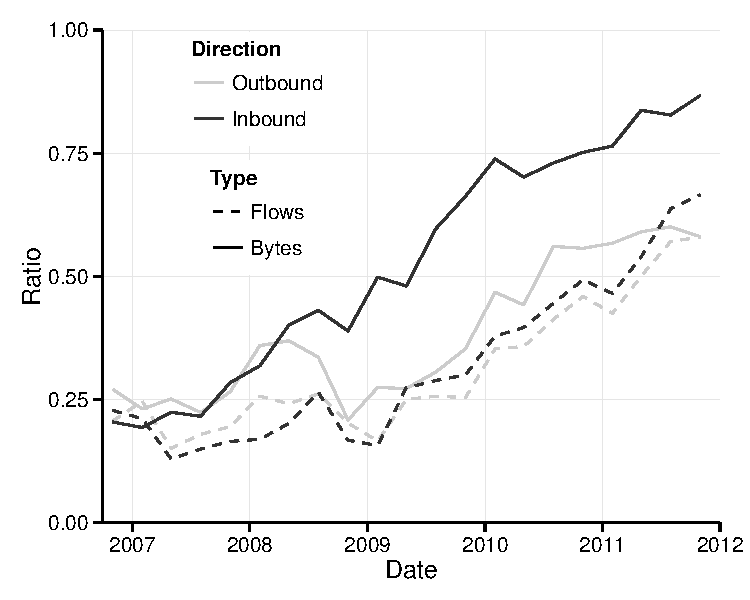
\includegraphics[width=2.5in]{figures/malawi/windowscale}
        \caption{\acs{TCP} windowscale deployment over time. \label{fig:windowscale}}
    \end{subfigure}%
    \begin{subfigure}[b]{.5\linewidth}
        \centering
        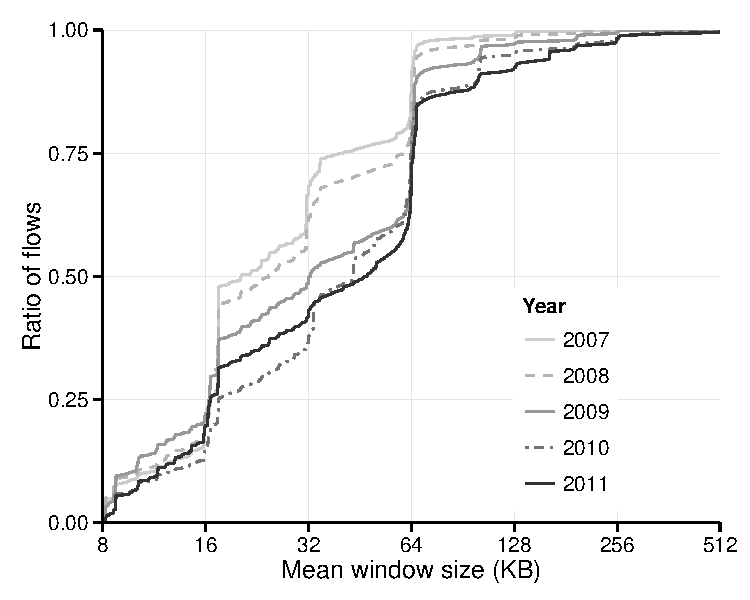
\includegraphics[width=2.5in]{figures/malawi/hostwindow}
        \caption{\acs{CDF} of window sizes for host limited flows.\label{fig:hostwindow}}
    \end{subfigure}%
    \caption{Longitudinal evolution of \acs{TCP} window parameters. \label{fig:tcpWindowParams}}
\end{figure}



\subsection{Throughput is primarily sender driven}

% define the assumption
A more widely held and less frequently enunciated assumption is that flow throughput is primarily determined at the sender side. 
Intuitively, it is in a receiver's best interests to maximize the flow rate, while the sender bears the responsibility for sharing network capacity and reducing the overhead incurred due to losses. 
The Internet architecture however confers the receiver the ability to throttle rates through flow control. 
From answering the previous assumption, it is clear that throughput \textit{is} mostly determined by the actions of the sender: receiver shaping and host limitations together affect at most 24\% of all traffic. 
Despite this it is worth understanding the nature of these host limitations in particular, and towards which direction flow control is swinging.

% explore the results
A critical component in determining the upper bound for the congestion window size is the negotiation of the \ac{TCP} \emph{windowscale} option during the initial handshake. 
In its absence, a sender cannot have more than 64KB in flight.
Furthermore, the \emph{default buffer size} on either end of the connection can also limit the size to which the congestion window can increase.
Both settings are primarily subject to operating system configuration.
Throughput conditions on the receiver side improve as \acs{OS} upgrades are rolled out.
The installed user base within \acs{WIDE} is comparatively stable over time, and as such is expected to exhibit continual improvements unless a significant \acs{OS} rollback were to occur or a large set of users with outdated \acp{OS} were to be added to the network.
This however is unlikely, and a more plausible explanation for any significant degradation in host limitations lies in macroscopic shifts in routing or application popularity which lead to a change in \emph{where} traffic originates from.

This hypothesis is tested by first verifying windowscale deployment over time.
Figure \ref{fig:windowscale} shows the ratio of traffic and flows for which windowscale was successfully negotiated.
Results are calculated solely over traffic where the initial handshake was observed.
For added context, data for the outbound direction is also displayed.
The first result that stands out is the steady increase over time of windowscale usage, rising from 25\% of all inbound bytes in early 2007 to almost 80\% by late 2011.
Furthermore, the effects of content consolidation manifest themselves in the disproportionate coverage of bytes when compared to flows.
With the reduced stake of large \acp{ISP} in inbound traffic, transit traffic has become dominated by a small set of centrally managed stakeholders such as Google, lowering the effective barrier for deployment of protocol extensions.
Conversely, the temporary drop in windowscale adoption for inbound flows in 2009 is due to the increase of traffic from Asian sources, in particular HiNet.

Given the prevalence of windowscaling, the primary source of host limitation should therefore be due to the configuration of socket buffer sizes.
Figure \ref{fig:hostwindow} shows the distribution of the average window size for flows which are flagged as being host limited.
While the 64KB limit intrinsic to \ac{TCP} is a common upper bound on window size, other defaults are apparent and have shifted over time.
The use of 16KB and 32KB buffer sizes (default buffer sizes for Windows XP and Vista respectively) was progressively phased out over the five year period.
In addition to traditional power-of-two increments of the window size, different limits are apparent amongst hosting providers: 50KB, 100KB (The Planet), 160KB (Limelight) and 200KB (SoftLayer), reflecting the overall weight such \acp{AS} can have in shaping transit traffic.
The influx of Asian traffic in 2009 led to an increase in observed host windows beneath 16KB.

\begin{table}\footnotesize
\centering
  \begin{subtable}[b]{.5\linewidth}
    \centering
    \begin{tabular}{  
    p{0.5cm} 
    >{\centering\arraybackslash}p{0.4cm} 
    >{\centering\arraybackslash}p{0.4cm} 
    >{\centering\arraybackslash}p{0.2cm} 
    >{\centering\arraybackslash}p{0.4cm} 
    >{\centering\arraybackslash}p{0.2cm} }

    & \multicolumn{2}{c}{ \textbf{Total (\%)}} & & \multicolumn{2}{c}{\textbf{Receiver (\%)}} \\
Year & Flows & Bytes & & Flows & Bytes \\

\hline

    2007 & 0.32 & 18.58 &  & 69.01 & 74.31\\2008 & 0.30 & 17.80 &  & 67.70 & 71.14\\2009 & 0.27 & 14.50 &  & 60.51 & 62.80\\2010 & 0.25 & 20.44 &  & 52.34 & 64.63\\2011 & 0.19 & 13.49 &  & 50.49 & 60.81
\\
    \bottomrule
    \end{tabular}
    \caption{Inbound traffic.}
  \end{subtable}%
  \begin{subtable}[b]{.5\linewidth}
    \centering
    \begin{tabular}{  
    p{0.5cm} 
    >{\centering\arraybackslash}p{0.4cm} 
    >{\centering\arraybackslash}p{0.4cm} 
    >{\centering\arraybackslash}p{0.2cm} 
    >{\centering\arraybackslash}p{0.4cm} 
    >{\centering\arraybackslash}p{0.2cm} }

    & \multicolumn{2}{c}{ \textbf{Total (\%)}} & & \multicolumn{2}{c}{\textbf{Receiver (\%)}} \\
Year & Flows & Bytes & & Flows & Bytes \\

\hline

    2007 & 8.22 & 24.24 &  & 76.50 & 82.54\\2008 & 11.80 & 32.40 &  & 68.81 & 84.38\\2009 & 10.40 & 30.50 &  & 62.50 & 84.28\\2010 & 4.00 & 27.00 &  & 76.14 & 88.07\\2011 & 3.01 & 25.94 &  & 72.00 & 85.91
\\
    \bottomrule
    \end{tabular}
    \caption{Outbound traffic.}
  \end{subtable}
  \caption[Percentage of host limited traffic over time.]{\label{table:hostlimited}Percentage of host limited traffic over time by total number of flows and bytes. The proportion for which the receiver side was the bottleneck is also shown.}
\end{table}

While figure \ref{fig:hostwindow} demonstrates that host limitations for inbound traffic have been lifted over time, it still does not adequately answer on what side of the connection they are imposed.
Table \ref{table:hostlimited} breaks down the proportion of host limited traffic over time for both inbound and outbound direction.
In addition to presenting the ratio of flows and bytes affected by host limitations, the relative proportion of traffic identified as being conditioned by the receiver side is also displayed.
In either direction a very small fraction of flows are affected.
Small flows are both numerous and unlikely to last long enough for window limits to be reached or reliably detected.
The affected flows therefore tend to be large, and as such can translate into a significant amount of traffic.
The proportion of flows and bytes for which the receiver side imposed the maximum window size dropped by 20\% and 15\% respectively over five years for inbound traffic, reflecting the successive \acs{OS} upgrades performed for hosts within \acs{WIDE}.
Interestingly, these trends do not surface for outbound traffic: hosts outside Japan were consistently more likely to dictate the maximum window size.
In part, this reflects the different nature of the traffic under observation: outbound traffic for this dataset is more geographically and topologically diverse, with content in many cases being retrieved from Japan by residential hosts from within Asia.

% summarize the answer
\textbf{The endpoint which ends up dictating the maximum achievable throughput through flow control is typically a function of the \acs{OS} adoption cycle.}
With the windowscale option covering 80\% of all inbound traffic, the main source of host level constraints are now conservative buffer sizes.
For this dataset, hosts internal to \acs{WIDE} have seemingly been upgraded at a faster rate, or less conservatively, than their remote counterpoints.
As such, throughput has become increasingly sender driven over time for inbound traffic.

\subsection{Throughput is correlated with flow size}

% define the assumption
Given host limitations are most likely to affect large flows, it's worth considering whether other constraints are applied disproportionately across flow sizes. 
A commonly held assumption is that throughput is correlated with flow size, which has been verified empirically in previous studies \cite{oursTCP, Zhang:2002p85}.
Much of the data used in these studies however precedes the widespread adoption of high bandwidth connections and use of streaming media, both of which can impact the extent to which contention occurs in the network.

\begin{figure}
    \begin{subfigure}[b]{.5\linewidth}
        \centering
        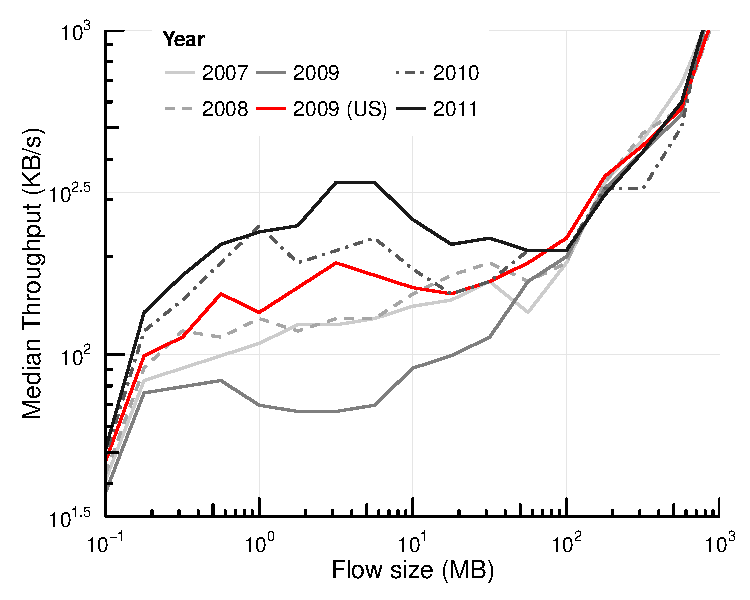
\includegraphics[width=2.5in]{figures/malawi/med_active_throughput}
        \caption{Mean congestion window over mean \ac{RTT}. \label{fig:flowrateactive}}
    \end{subfigure}%
    \begin{subfigure}[b]{.5\linewidth}
        \centering
        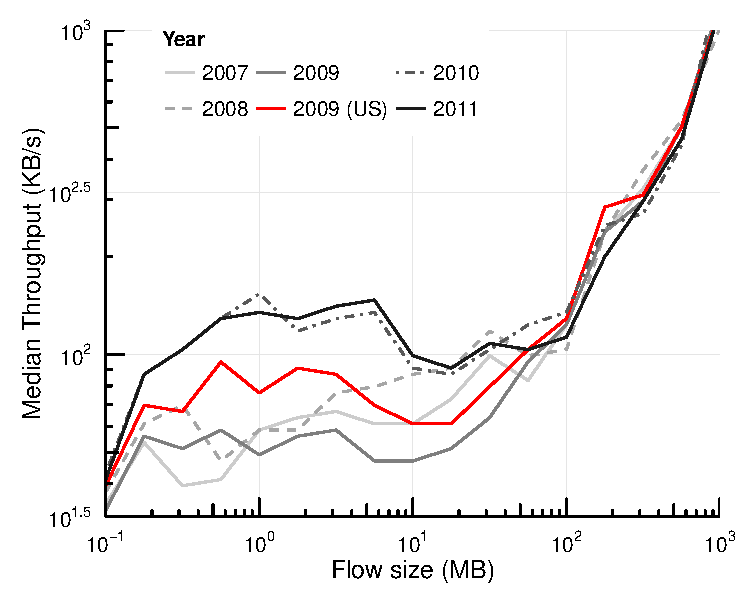
\includegraphics[width=2.5in]{figures/malawi/med_aggr_throughput}
        \caption{Flow size over flow duration.\label{fig:flowrateaggr}}
    \end{subfigure}%
    \caption{Median throughput for inbound traffic by flow size. \label{fig:flowrate}}
\end{figure}
 
% explore the results
Figure \ref{fig:flowrate} shows the median throughput as a function of flow size, by year.
In figure \ref{fig:flowrateactive}, flow throughput is calculated as the ratio between the mean \ac{TCP} window size (in bytes) and the mean flight length (in seconds).
Compared to the more commonly used ratio of flow size by flow duration, displayed in figure \ref{fig:flowrateaggr}, this method is less susceptible to application behaviour and as such provides a more accurate estimate of the achievable rate.
In both cases, flows are binned by size on a logarithmic scale, with median throughput calculated across each bin.
Due to routing changes and increased congestion, overall throughput in 2009 is lower than other years given there is a greater proportion of traffic from Asian neighbours, particularly over smaller flow sizes.
For reference the throughput for traffic from the US alone is plotted for 2009,in which case a more natural yearly progression becomes apparent.
For both plots, a clear disparity is visible across flows sizes: for flows in the 10MB to 100MB range, although throughput has consistently increased with time, it has done so at a lower pace than for flows under 10MB. 

\begin{figure}
    \begin{subfigure}[b]{.5\linewidth}
        \centering
        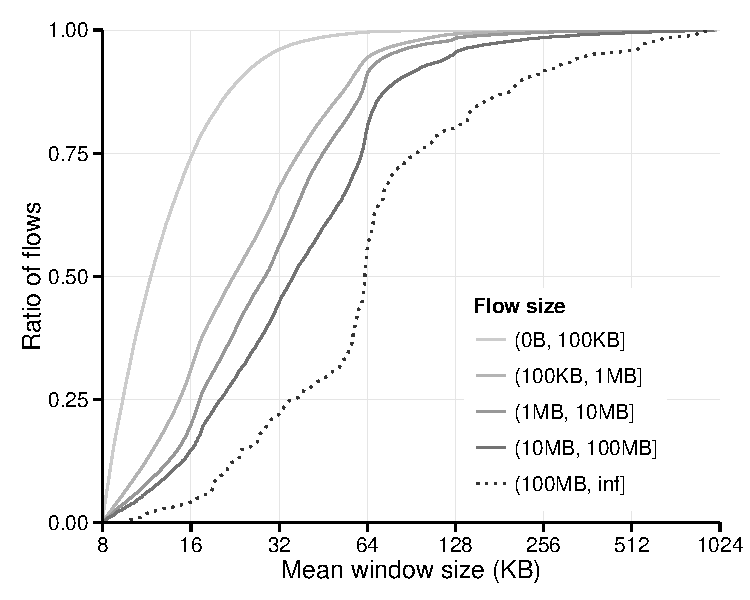
\includegraphics[width=2.5in]{figures/malawi/windowsize2007}
        \caption{2007.}
    \end{subfigure}%
    \begin{subfigure}[b]{.5\linewidth}
        \centering
        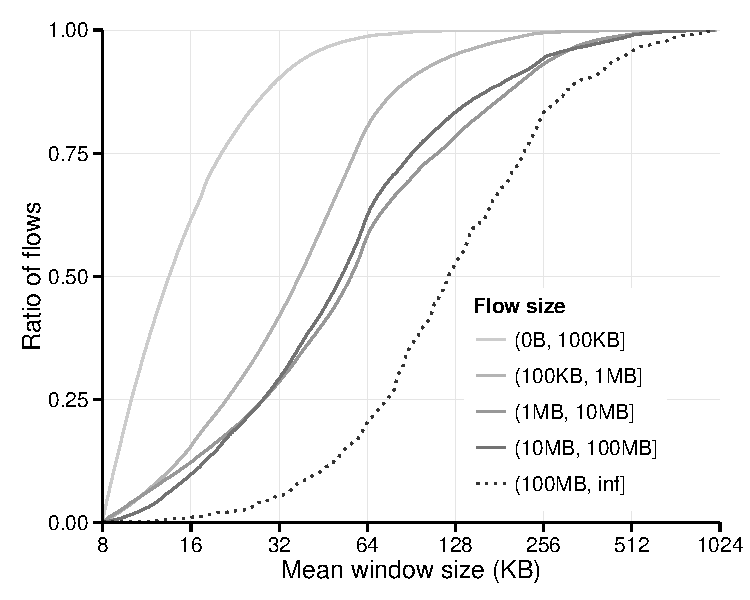
\includegraphics[width=2.5in]{figures/malawi/windowsize2011}
        \caption{2011.}
    \end{subfigure}%
    \caption{\acs{CDF} of the average window size by flow size by year. \label{fig:windowsize}}
\end{figure}
 
These results confirm the notion that the highest throughputs are attained by the largest flows, but they also show that improvements in throughput do not apply equally to all flow sizes. 
Whereas throughput has consistently improved for low-volume traffic, it has not done so for high-volume traffic. 
Hence, these findings suggest an increased differentiation between high-value, low-volume traffic whose throughput has markedly increased, and low-value, high-volume traffic whose throughput has stagnated.
Although the reported flow sizes are not a reliable predictor of the overall traffic volume amassed over a flow's lifetime given the short time span of each daily trace, this seemingly subverts the notion that flow rates are strongly correlated with flow size in a simple, proportional fashion.  
This is expounded by further analysing the average window sizes across flow sizes, displayed in Figure \ref{fig:windowsize}.
In 2007, there is a visible correlation, with larger flows attaining higher window sizes.
Furthermore, the distributions cluster prominently around 64KB due to a low rate of windowscale negotiation.
By 2011, this clustering is less pronounced, with window sizes increasing across the board, but with larger flows often outpaced by shorter counterparts.

% compare aggr vs active


\begin{table}\footnotesize
\centering
  \begin{subtable}[b]{1.0\linewidth}
    \centering
    \begin{tabular}{  p{1.0cm} 
>{\centering\arraybackslash}p{1.0cm} 
>{\centering\arraybackslash}p{1.0cm} 
>{\centering\arraybackslash}p{1.0cm} 
>{\bfseries\centering\arraybackslash}p{1.0cm} 
>{\centering\arraybackslash}p{1.0cm} }

& \multicolumn{4}{c}{Limitation (\%)} \\
\cline{2-5}
Year & Application & Host & Receiver & Total & Loss (\%)\\

\hline

    2007 & 14.65 & 5.45 & 0.10 & 20.20 & 1.90 \\2008 & 14.99 & 5.37 & 0.09 & 20.44 & 2.27 \\2009 & 15.66 & 3.83 & 0.55 & 20.03 & 2.39 \\2010 & 10.55 & 4.18 & 0.36 & 15.09 & 2.15 \\2011 & 11.13 & 2.53 & 0.05 & 13.71 & 1.19 \\

    \bottomrule
    \end{tabular}
  \caption{Flows under 10MB.}
  \end{subtable}
  \begin{subtable}[b]{1.0\linewidth}
    \centering
    \begin{tabular}{  p{1.0cm} 
>{\centering\arraybackslash}p{1.0cm} 
>{\centering\arraybackslash}p{1.0cm} 
>{\centering\arraybackslash}p{1.0cm} 
>{\bfseries\centering\arraybackslash}p{1.0cm} 
>{\centering\arraybackslash}p{1.0cm} }

& \multicolumn{4}{c}{Limitation (\%)} \\
\cline{2-5}
Year & Application & Host & Receiver & Total & Loss (\%)\\

\hline

    2007 & 0.96 & 61.62 & 23.07 & 0.71 & 85.40 \\2008 & 0.88 & 61.49 & 21.94 & 0.92 & 84.35 \\2009 & 0.98 & 57.86 & 17.70 & 3.28 & 78.85 \\2010 & 0.71 & 43.97 & 24.45 & 4.03 & 72.45 \\2011 & 0.62 & 52.95 & 15.55 & 0.71 & 69.21 \\

    \bottomrule
    \end{tabular}
  \caption{Flows over 10MB.}
  \end{subtable}
\caption[Percentage of traffic in bytes affected by each constraint by year according to flow size.]{Percentage of traffic in bytes affected by each constraint by year according to flow size, along with aggregate retransmission ratio.}
\label{table:full}
\end{table}

Clearly, the extent to which rates are constrained is closely tied to flow size. 
Table \ref{table:full} breaks down the results from table \ref{table:limits} by flow size. 
Most limitations will invariably affect larger flows, as applications which shift more traffic, such as streaming media or bulk file transfers, are more likely to either attain or self-impose constraints on flow throughput. 
Many small flows on the other hand never exit slow start, in which case none of the studied constraints will be reached or readily identified. 
This dichotomy is reflected on loss rates, which will be higher for flows regulated by \ac{TCP} congestion control.
Additionally, the discrepancy in loss rates is further exacerbated by geographic properties: traffic exchanged over poor infrastructure tends to be smaller, with flows from China exhibiting particularly high end-to-end loss rates. 

\textbf{These results suggest that network upgrades are unlikely to improve performance for significant proportions of traffic.} 
This is most visible in figure \ref{fig:flowrate}, where improvements in capacity for coping with higher bursts of activity (figure \ref{fig:flowrateactive}) has outpaced the actual delivery rate set by applications (figure \ref{fig:flowrateaggr}).
Given the popularity of emulating a constant bit rate service over \ac{TCP}, that no such abstraction is provided at the socket level \acs{API} is unfortunate.


\subsection{Throttling primarily affects heavy hitters}

% define the assumption
The observations so far have highlighted that flow throughput is often subjugated from \ac{TCP} by external stakeholders.
A third important element in the ensuing tussle is in understanding the role operators can play in imposing their own preferences upon traffic.
As such, this section provides a brief overview of the extent, and under what circumstances, customer networks resorted to receiver shaping over the duration of the dataset.
From preliminary inspection of table \ref{table:full}, it is apparent that receiver shaping was limited in both scope, affecting at most 4\% of bytes, and time, being primarily concentrated within 2009 and 2010.
A breakdown of receiver shaping by traffic source is provided in table \ref{table:toprecvlim}, listing for each year the five most affected stakeholders within the top twenty \acp{AS}, and their respective contribution to the overall traffic and retransmissions observed yearly.

% explore the results
\begin{table}[t]
\footnotesize
\centering
\begin{tabular}{
rr 
>{\raggedright}p{2.1cm}
>{\bfseries\raggedleft}p{1.2cm}
>{\raggedleft}p{0.8cm}
>{\raggedleft\arraybackslash}p{0.8cm}}

& & & \textmd{Limitation} & \multicolumn{2}{c}{(\%) of total } \\
\cline{5-6}
Year & ASN & AS Name & Receiver & Bytes & Rexmt \\
\hline

2007
 & 8071 & Microsoft & 4.61 & 0.69 & 0.17 \\ & 41690 & DailyMotion & 2.57 & 0.52 & 0.13 \\ & 20940 & Akamai & 1.50 & 1.49 & 0.90 \\ & 22822 & Limelight & 1.37 & 8.12 & 5.01 \\ & 19166 & ACRONOC & 0.81 & 1.40 & 1.22 \\

\ASLISTSEP{2008}
 & 21844 & The Planet & 2.43 & 0.76 & 0.82 \\ & 174 & Cogent & 2.02 & 1.89 & 1.39 \\ & 19166 & ACRONOC & 1.61 & 2.02 & 1.16 \\ & 1299 & TeliaNet & 1.25 & 1.25 & 1.59 \\ & 2914 & NTT & 1.03 & 17.16 & 13.24 \\

\ASLISTSEP{2009}
 & 16276 & OVH & 31.97 & 1.26 & 0.29 \\ & 3356 & Level 3 & 6.24 & 2.18 & 1.50 \\ & 22822 & Limelight & 5.92 & 1.60 & 0.88 \\ & 174 & Cogent & 5.49 & 1.30 & 0.91 \\ & 16265 & LeaseWeb & 5.09 & 1.98 & 1.06 \\

\ASLISTSEP{2010}
 & 1299 & TeliaNet & 25.67 & 1.31 & 1.43 \\ & 3356 & Level 3 & 17.33 & 2.71 & 3.16 \\ & 16276 & OVH & 15.28 & 1.84 & 0.32 \\ & 16265 & LeaseWeb & 7.70 & 3.23 & 2.16 \\ & 29748 & Carpathia (Ashburn) & 7.46 & 2.62 & 1.30 \\

\ASLISTSEP{2011}
 & 7366 & Lemuria & 4.45 & 1.96 & 1.56 \\ & 46742 & Carpathia (LAX) & 1.89 & 1.64 & 0.68 \\ & 46179 & Mediafire & 1.20 & 1.54 & 0.82 \\ & 29748 & Carpathia (Ashburn) & 1.08 & 2.06 & 1.27 \\ & 35415 & Webazilla & 0.95 & 6.05 & 3.33 \\

\bottomrule
\end{tabular}
\caption[\acs{AS}-level analysis of receiver shaping.]{\acs{AS}-level analysis of receiver shaping. For each year, the five most affected \acp{AS} are listed with the total proportion of traffic which was receiver shaped as well as the overall contribution of the \ac{AS} to the total volume of bytes and retransmissions for that year.\label{table:toprecvlim}}
\end{table}

Prior to 2009, receiver shaping mostly targeted flows which attained the highest throughput, and may have in part been performed by hosts. 
In addition to affecting Microsoft, which distributes Windows updates using the same flow control mechanisms exploited by middleboxes, some \ac{CDN} traffic was also reined in.
By 2009, and likely as a reaction to increased contention within their networks, the network-level footprint of receiver side throttling shifts from shaping by rate, to shaping by volume.
Specific targets start to emerge within OVH, Cogent and Level 3 and TeliaNet, all of which hosted significant file-sharing websites at the time which would continue to be affected throughout 2010.
By 2011, receiver shaping mostly subsided, affecting primarily Lemuria (HotFile) and Mediafire.
In the presence of increased contention, some customer networks felt obliged to curb traffic which in many cases was already limited by the source.
The selected targets of shaping however were neither the biggest contributors in terms of volume, nor the most aggressive senders as reflected by the relative proportion of retransmissions, most likely being singled out instead based on the perceived legality of the content downloaded.
When consulting the overall popularity of these targets in table \ref{table:topapplim}, it is apparent that some of the most throttled \acp{AS} such as Carpathia and Lemuria had been far more popular in previous years, suggesting that users may migrate to other content providers when confronted with lower rates.
While successive bandwidth upgrades alleviated the need for throttling, it is unclear whether the middleboxes responsible were discontinued, or limits were merely raised to the extent where the sender side would once again become the bottleneck.

% summarize the answer
\textbf{In some cases, multiple stakeholders apply different rate control mechanisms simultaneously, leading to quality degradation and unusual rate behaviours.}
Conventionally, it is assumed that it is in the best interest of content providers to use network resources as fully as possible, whereas \acp{ISP} have it in their best interest to police resource usage and control flow rates. 
However, as shown here, current business practices can create an alignment of incentives where both content providers and \acp{ISP} choose to limit the throughput of a particular class of traffic. 
This may lead to traffic suffering from artificially slow rates that are much worse than those experienced by other classes. 
In these cases, the combination of multiple rate control techniques being applied by different stakeholders may lead to a traffic profile whose rate behaves in a manner quite removed from the commonly assumed \ac{TCP} dynamics.

